\subsubsection{Gravity field generated by mantle density variations}
\label{sec:benchmark-mantle-gravity}

\textit{This section was contributed by C. Thieulot and L. Jeanniot.}

The gravity postprocessor has been benchmarked in Section~\ref{sec:benchmark-thin-shell-gravity} and \ref{sec:benchmark-thick-shell-gravity}.
We use it here in an Earth-like context: the tomography model S40RTS \cite{S40RTS} is used and scaled so as to provide temperature anomalies, which themselves incorporated in the Simple material model yield a density distribution for the entire Earth mantle minus the lithosphere, i.e. $R\textsubscript{inner} \leq r \leq R\textsubscript{outer}$  with $R\textsubscript{inner}=3480~\si{\km}$ and $R\textsubscript{outer}=6251~\si{\km}$. The use of the S20RTS/S40RTS tomography model and its parameterization is detailed in Section~\ref{sec:cookbooks-S20RTS}.

We set the global refinement to 3 so that the mesh counts $12\times 16^3=49,152$ cells. This means that the radial resolution is $(R\textsubscript{outer}-R\textsubscript{inner})/16\simeq  173~\si{\km}$ while the lateral resolution is $(4\pi R\textsubscript{outer}^2/(12\times 16^2))^{1/2} \simeq 400~\si{km}$ at the surface and $(4\pi R\textsubscript{inner}^2/(12\times 16^2))^{1/2} \simeq 220~\si{km}$ at the CMB. The mesh and the density field are shown in Fig.~\ref{fig:grav_mantle1}. The temperature anomaly ranges from approximately $-342~\si{\kelvin}$ to approximately $+331~\si{\kelvin}$ and geodynamical features such as the mid-oceanic ridge or the Afar region are visible in the form of positive temperature anomalies, indicating that mantle material is present in these areas. Note that these values are not necessarily meaningful since we here assume that density variations are 100\% due to temperature variations as there is only a single material in the domain (i.e. no change in composition in space). Nevertheless this simple setup provides us with a complex-enough density distribution to test the gravity postprocessor.

\begin{figure}
  \centering
  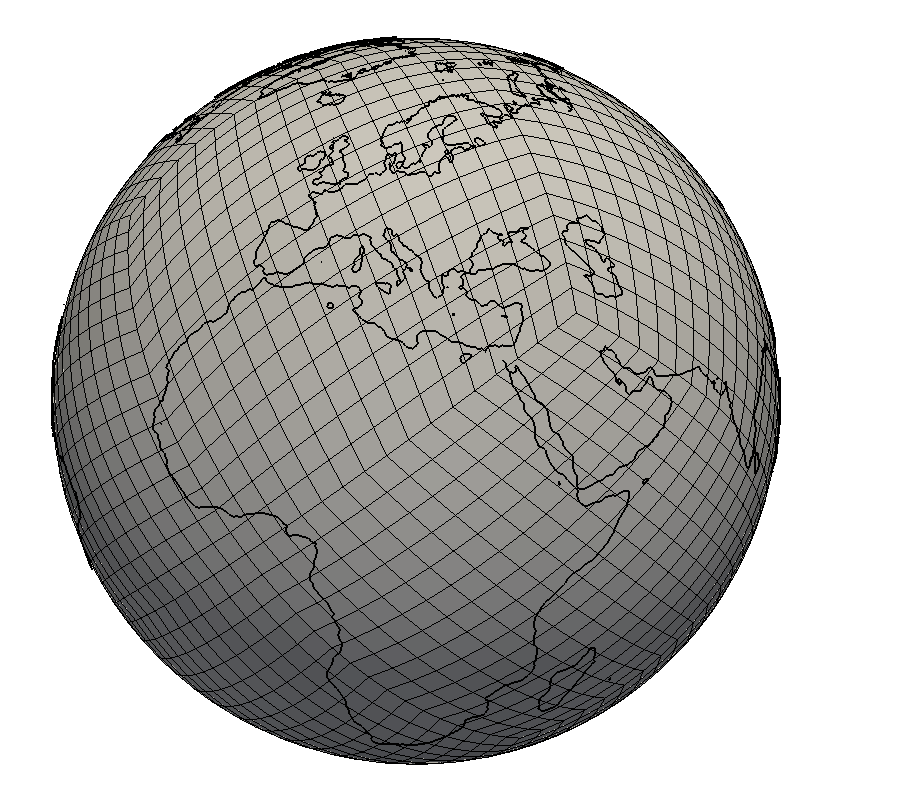
\includegraphics[width=5cm]{cookbooks/benchmarks/gravity_mantle/doc/mesh}
  \hfill
  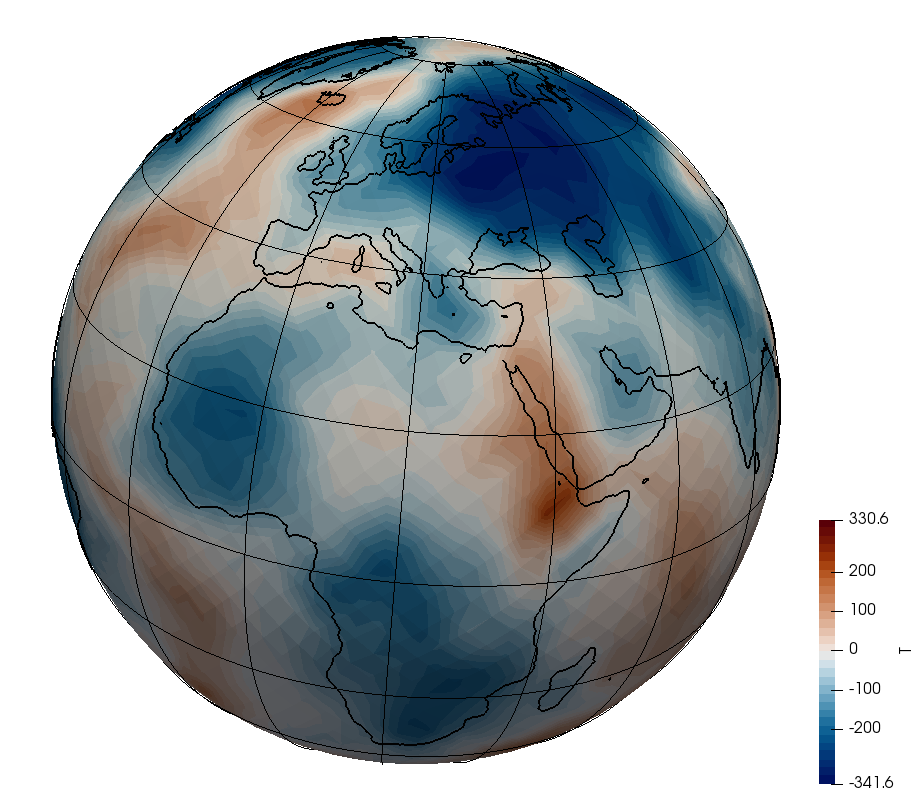
\includegraphics[width=5cm]{cookbooks/benchmarks/gravity_mantle/doc/T}
  \hfill
  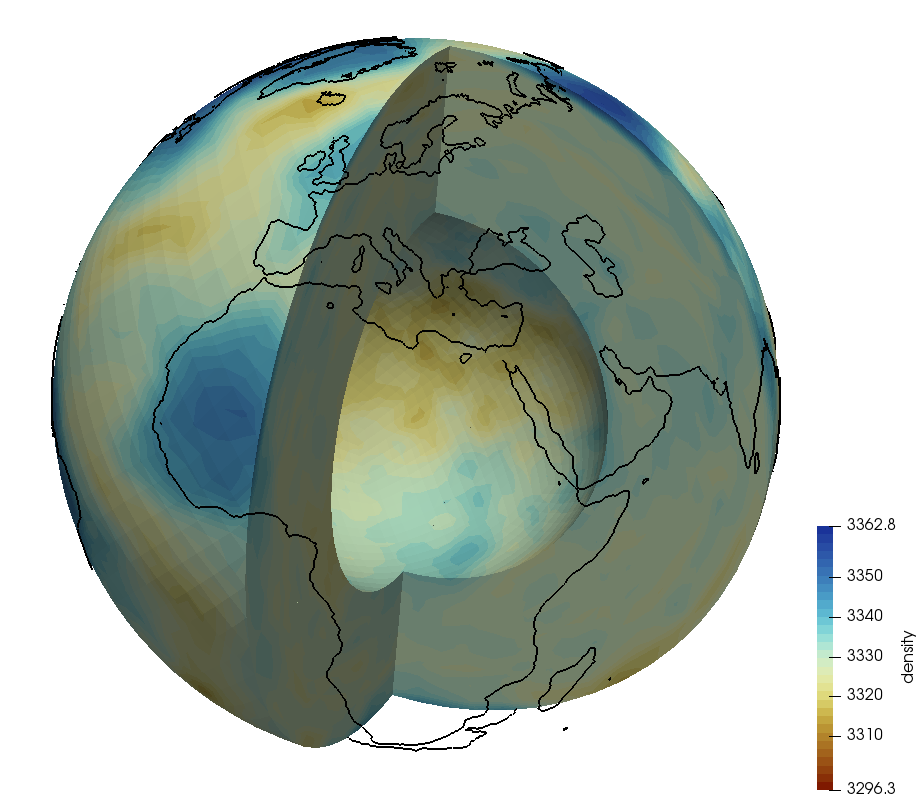
\includegraphics[width=5cm]{cookbooks/benchmarks/gravity_mantle/doc/rho}
  \caption{Mantle gravity cookbook. From left to right: mesh, temperature anomaly and density. Coastlines are available for Paraview at 
\url{https://www.earthmodels.org/date-and-tools/coastlines/los-alamos}. Once opened the data must be scaled up (simply set the scale of the lower left menu in Paraview to the desired outer radius of your model). Grid lines are also available on the same site.}
  \label{fig:grav_mantle1}
\end{figure}

The gravity postprocessor computes the gravitational potential, acceleration vector and gradient at a given radius (here chosen to be $6371+250=6621~\si{\km}$) on a regular $2\si{\degree}$-latitude-longitude grid (see also the cookbook of Section~\ref{sec:benchmark-thin-shell-gravity}) and returns the results in the \texttt{gravity-00000} file to be found in the \texttt{output-gravity} folder inside the regular output folder. 

The python script \texttt{convert\_gravity\_ascii\_to\_vtu\_map.py} converts the ascii output to \texttt{vtu} format in order to view the results in ParaView. It is provided in the folder of this cookbook and can be used as follows:
\begin{lstlisting}[frame=single,language=ksh,showstringspaces=false]
python3 convert_gravity_ascii_to_vtu_map.py gravity-00000 181 91
\end{lstlisting}
The first argument is the ascii file, while the following two arguments are the number of longitude and latitude points as specified in the \texttt{prm} file.
The resulting \texttt{gravity-00000\_map.vtu} file is then visualised with ParaView and is shown in Fig.~\ref{fig:grav_mantle2}. Note that on a modern laptop the calculations resulting from running the provided \texttt{prm} file in the cookbook folder takes a bit less than 2 hours on a single thread: about 1250~\si{\second} are spent in the setup phase (using the spherical harmonics coefficients to compute the temperature field on the mesh nodes) and about 4700~\si{\second} in the gravity postprocessor itself. This time can be substantially decreased by running \aspect{} in parallel on $n$ threads: the processor can then make use of the domain decomposition and is almost $n$ times faster.

As shown in the thin shell gravity benchmark the constant component of the density $\rho_0=3300~\si{\kg\per\cubic\metre}$ generates a constant gravity field at the measurement radius so it can be filtered out. In general, the contribution to the gravity signal of any density distribution that solely depends on $r$ can and should be removed as it does not contain any valuable information.


\begin{figure}
  \centering
  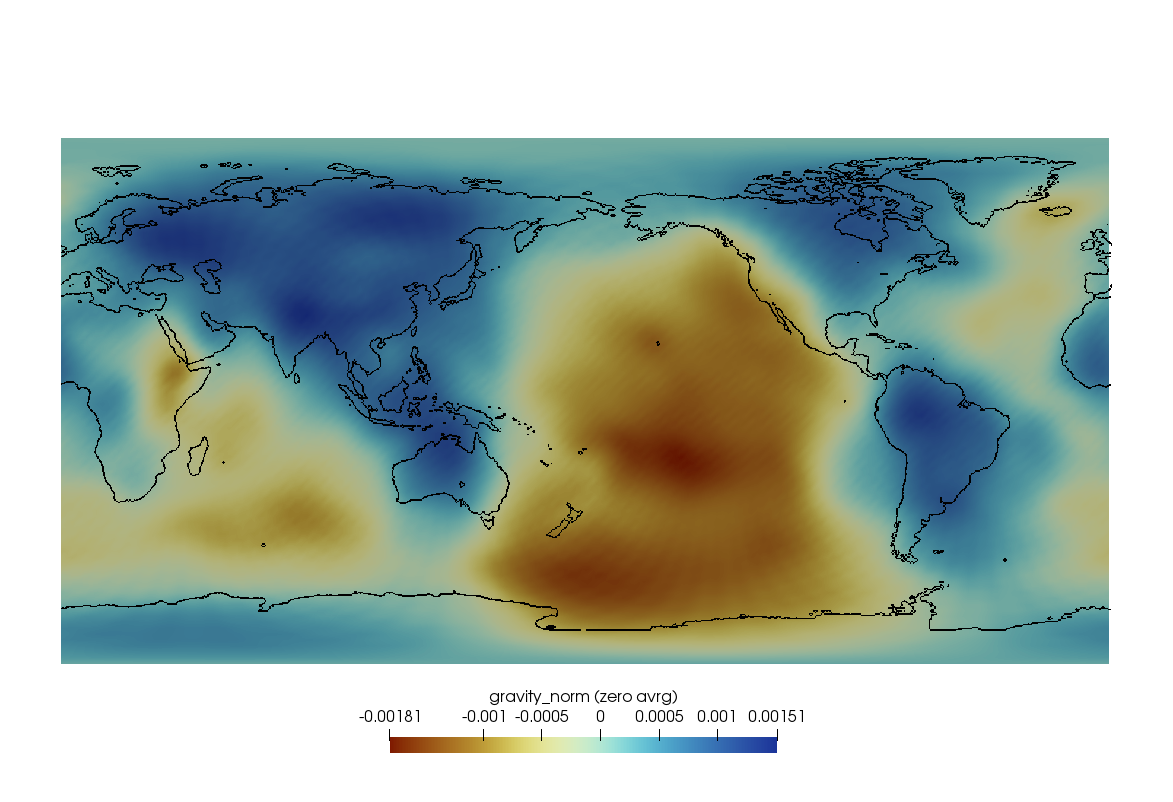
\includegraphics[width=0.48\textwidth]{cookbooks/benchmarks/gravity_mantle/doc/grav}
  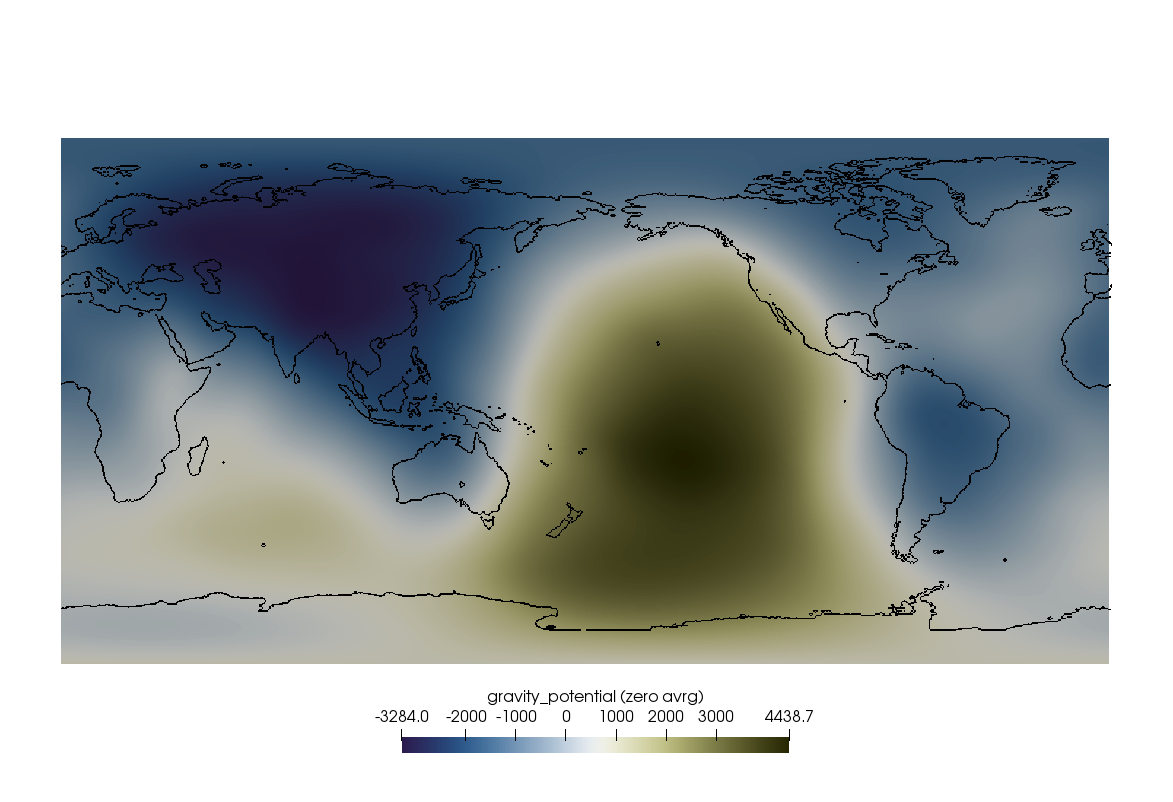
\includegraphics[width=0.48\textwidth]{cookbooks/benchmarks/gravity_mantle/doc/pot}
  \caption{Mantle gravity: gravitational acceleration $|g|$ (left) and potential (right) computed at radius 6621~\si{\km}.}
  \label{fig:grav_mantle2}
\end{figure}


